\documentclass[]{article}
\usepackage{graphicx}
\usepackage[svgnames]{xcolor} 
\usepackage{fancyhdr}
\usepackage{tocloft}
\usepackage[hidelinks]{hyperref}
\usepackage{enumitem}
\usepackage[many]{tcolorbox}
\usepackage{listings }
%\usepackage[a4paper, total={6in, 8in} , top = 2cm,bottom = 4cm]{geometry}
\usepackage[a4paper, total={6in, 8in}]{geometry}
\usepackage{afterpage}
\usepackage{amssymb}
\usepackage{pdflscape}
\usepackage{textcomp}
\usepackage{xecolor}
\usepackage{rotating}
\usepackage[Kashida]{xepersian}
\usepackage[T1]{fontenc}
\usepackage{tikz}
\usepackage[utf8]{inputenc}
\usepackage{PTSerif} 
\usepackage{seqsplit}
\usepackage{changepage}


\usepackage{listings}
\usepackage{xcolor}
\usepackage{sectsty}

\setcounter{secnumdepth}{0}
 
\definecolor{codegreen}{rgb}{0,0.6,0}
\definecolor{codegray}{rgb}{0.5,0.5,0.5}
\definecolor{codepurple}{rgb}{0.58,0,0.82}
\definecolor{backcolour}{rgb}{0.95,0.95,0.92}
\definecolor{blanchedalmond}{rgb}{1.0, 0.92, 0.8}
\definecolor{brilliantlavender}{rgb}{0.96, 0.73, 1.0}
\definecolor{CustomColor}{HTML}{cc0000}
 
\NewDocumentCommand{\codeword}{v}{
\texttt{\textcolor{blue}{#1}}
}
\lstset{language=java,keywordstyle={\bfseries \color{blue}}}

\lstdefinestyle{mystyle}{
    backgroundcolor=\color{backcolour},   
    commentstyle=\color{codegreen},
    keywordstyle=\color{magenta},
    numberstyle=\tiny\color{codegray},
    stringstyle=\color{codepurple},
    basicstyle=\ttfamily\normalsize,
    breakatwhitespace=false,         
    breaklines=true,                 
    captionpos=b,                    
    keepspaces=true,                 
    numbers=left,                    
    numbersep=5pt,                  
    showspaces=false,                
    showstringspaces=false,
    showtabs=false,                  
    tabsize=2
}

\lstset{style=mystyle}

 \settextfont[BoldFont={XB Zar bold.ttf}]{XB Zar.ttf}


\setlatintextfont[Scale=1.0,
 BoldFont={LiberationSerif-Bold.ttf}, 
 ItalicFont={LiberationSerif-Italic.ttf}]{LiberationSerif-Regular.ttf}





\newcommand{\inputsample}[1]{
    ~\\
    \textbf{ورودی نمونه}
    ~\\
    \begin{tcolorbox}[breakable,boxrule=0pt]
        \begin{latin}
            \large{
                #1
            }
        \end{latin}
    \end{tcolorbox}
}

\newcommand{\outputsample}[1]{
    ~\\
    \textbf{خروجی نمونه}

    \begin{tcolorbox}[breakable,boxrule=0pt]
        \begin{latin}
            \large{
                #1
            }
        \end{latin}
    \end{tcolorbox}
}

\newtcolorbox{mybox}[2][]{colback=red!5!white,
colframe=red!75!black,fonttitle=\bfseries,
colbacktitle=red!85!black,enhanced,
attach boxed title to top center={yshift=-2mm},
title=#2,#1}

\newenvironment{changemargin}[2]{%
\begin{list}{}{%
\setlength{\topsep}{0pt}%
\setlength{\leftmargin}{#1}%
\setlength{\rightmargin}{#2}%
\setlength{\listparindent}{\parindent}%
\setlength{\itemindent}{\parindent}%
\setlength{\parsep}{\parskip}%
}%
\item[]}{\end{list}}


\definecolor{foldercolor}{RGB}{124,166,198}
\definecolor{sectionColor}{HTML}{ff5e0e}
\definecolor{subsectionColor}{HTML}{008575}

\definecolor{listColor}{HTML}{00d3b9}

\definecolor{umlrelcolor}{HTML}{3c78d8}

\definecolor{subsubsectionColor}{HTML}{3c78d8}

\defpersianfont\authorFont[Scale=0.9]{XB Zar bold.ttf}

\defpersianfont\titr[Scale=1.5]{Lalezar-Regular.ttf}

\defpersianfont\fehrest[Scale=1.2]{Lalezar-Regular.ttf}

\defpersianfont\fehrestTitle[Scale=3.0]{Lalezar-Regular.ttf}

\defpersianfont\fehrestContent[Scale=1.2]{XB Zar bold.ttf}


\sectionfont{\color{sectionColor}}  % sets colour of sections
\subsectionfont{\color{subsectionColor}}  % sets colour of sections
\subsubsectionfont{\color{subsubsectionColor}}


\renewcommand{\labelitemii}{$\circ$}


\renewcommand{\baselinestretch}{1.1}


\renewcommand{\contentsname}{فهرست}

\renewcommand{\cfttoctitlefont}{\fehrestTitle}


\renewcommand\cftsecfont{\color{sectionColor}\fehrestContent\selectfont}
\renewcommand\cftsubsecfont{\color{subsectionColor}\fehrestContent\selectfont}
\renewcommand\cftsubsubsecfont{\color{subsubsectionColor}\fehrestContent\selectfont}
\renewcommand{\cftsecleader}{\cftdotfill{\cftdotsep}}
%\renewcommand{\cftsecpagefont}{\color{sectionColor}}

\setlength{\parskip}{1.2pt}

\begin{document}


%%% title pages
\begin{titlepage}
\begin{center}

\textbf{ \Huge{به نام خدا} }
        
\vspace{0.2cm}


\includegraphics[width=0.4\textwidth]{sharif1.png}\\
\vspace{0.2cm}
\textbf{ \Huge{\emph درس برنامه‌سازی پیشرفته} }\\
\vspace{0.25cm}
\textbf{ \Large{شبکه} }
\vspace{0.2cm}
       
 
      \large \textbf{دانشکده مهندسی کامپیوتر}\\\vspace{0.1cm}
    \large   دانشگاه صنعتی شریف\\\vspace{0.2cm}
       \large   ﻧﯿﻢ سال دوم 99-98 \\\vspace{0.10cm}
      \noindent\rule[1ex]{\linewidth}{1pt}
اساتید:\\
    \textbf{{مهدی مصطفی‌زاده، ایمان عیسی‌زاده، امیر ملک‌زاده، علی چکاه}}



        \vspace{0.10cm}
نگارش و تهیه محتوا:\\
    \textbf{{علیرضا ضیایی، سجاد ریحانی، محسن دهقان کار}}
    
       \vspace{0.10cm}
       تنظیم داک:\\
    \textbf{{امیرمهدی نامجو}}

    
        \vspace{0.05cm}
    

\end{center}
\end{titlepage}
%%% title pages


%%% header of pages
\newpage
\pagestyle{fancy}
\fancyhf{}
\fancyfoot{}
\cfoot{\thepage}
\lhead{شبکه}
\rhead{
\includegraphics[width=0.1\textwidth]{sharif.png}\\
دانشکده مهندسی کامپیوتر
}
\chead{پروژه برنامه‌سازی پیشرفته}
%%% header of pages
\renewcommand{\headrulewidth}{2pt}

\KashidaOff



\tableofcontents

\newpage

 \Large \textbf{\\\\
}

\section*{{\titr شبکه چیست؟}}
\addcontentsline{toc}{section}{{\fehrestContent شبکه چیست؟}}

به مجموعه‌ای از کامپیوتر‌های متصل به هم و زیر ساخت‌های ارتباطی(مانند \lr{Switch}، \lr{Router}، \lr{Firewall} و …) آن‌ها یک شبکه گفته می‌شود. بزرگ‌ترین شبکه کامپیوتری در جهان همین اینترنت است.


\section*{{\titr لایه‌های شبکه}}
\addcontentsline{toc}{section}{{\fehrestContent لایه‌های شبکه}}

شبکه‌های کامپیوتری (مثل اینترنت)  پیچیدگی‌های زیادی دارند، به همین خاطر برای توصیف آن‌ها از لایه بندی شبکه استفاده می‌شود. به این صورت که شبکه و پروتکل‌های آن را به صورت یک سری لایه بررسی می‌کنند که هر لایه از سرویسی که لایه زیرینش فراهم می‌کند استفاده کرده و سرویسی را به لایه‌ی بالاتر خود ارائه می‌دهد.

برای روشن شدن لایه‌های شبکه به این مثال توجه کنید. ما روزانه با سیستم‌های پیچیده‌ای سروکار داریم. فرض کنید فردی از شما می‌خواهد که برایش سیستم حمل و نقل هوایی را توصیف کنید. یکی از شیوه‌های توصیف این سیستم می‌تواند این گونه باشد که کارهایی را که یک فرد تا رفتن به مقصد باید انجام دهد را لیست کنیم.

 مثلا ابتدا بلیط تهیه می‌کنیم، چمدان‌هایمان چک می‌شوند، به گیت می‌رویم و نهایتا سوار هواپیما می شویم. سپس هواپیما پرواز می‌کند و مسیرش را تا مقصد می‌پیماید. بعد از فرود آمدن هواپیما، به گیت می‌رویم، چمدان‌هایمان را می‌گیریم. این سناریو در تصویر زیر خلاصه می‌شود.

\begin{center}
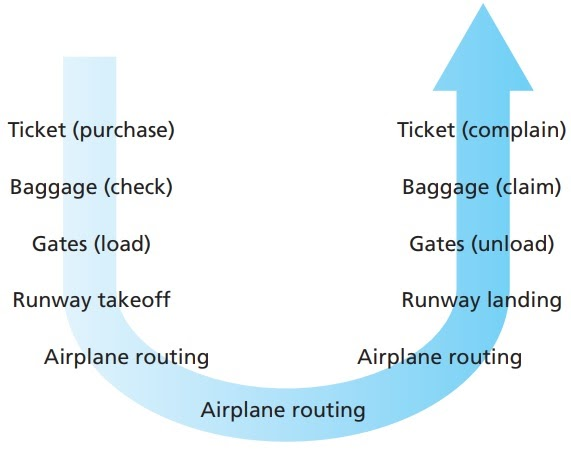
\includegraphics[width=0.5\textwidth]{images/1.jpg}
\end{center}

اتفاقی که در شبکه می‌افتد این است که تعدادی بسته اطلاعات (\lr{data packets}) قرار است از کامپیوتر مبدا به مقصد بروند. همان طور که مشهود است، این کار شباهت‌هایی با سفر با هواپیما دارد.

 
آنچه در توصیف هواپیما گفتیم را به‌خاطر بیاورید، با توجه به شکل زیر این فرایند را بگونه‌ای دیگر نمایش می‌دهیم. دقت کنید که:


\begin{itemize}
\item
برای سوار شدن هواپیما باید فرآیند خرید بلیط را انجام دهیم (\lr{ticketing function}) سپس از طرف دیگر هنگام پیاده شدن از هواپیما در مقصد نیز بلیط چک می‌شود (‌\lr{ticketing function}). 
\item
قبل از سوار شدن در هواپیما (مبدا) ، چمدان‌هایمان را تحویل می‌دهیم (\lr{baggage function}) و از سوی دیگر در شهر مقصد چمدان‌هایمان را تحویل می‌گیریم (\lr{baggage function})

\item
...

\begin{center}
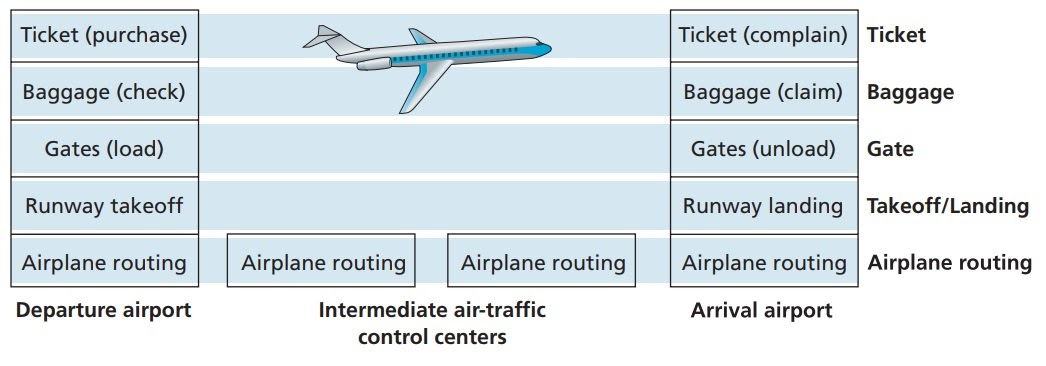
\includegraphics[width=0.7\textwidth]{images/2.jpg}
\end{center}
\end{itemize}

با توجه به این شکل، سفر با هواپیما ساختار خاصی پیدا می‌کند و ما می‌توانیم کارهای مختلفی را که انجام می‌دهیم (مثلا کارهای مربوط به تهیه و نشان دادن بلیط‌) به شکل افقی یا لایه‌ای توصیف کنیم. مثلا کارهای مربوط به بلیط یک لایه هستند و کارهای مربوط به \lr{baggage} یک لایه دیگر محسوب می‌شوند.

اگر دقت کنید، هر لایه همراه با لایه‌های زیرین خود به نوعی یک عملکرد و سرویس را پیاده سازی می‌کند. مثلا لایه‌ی بلیط به همراه لایه‌های زیرین، کار انتقال مسافر از پیشخوان یک فرودگاه به پیشخوان فرودگاه دیگر را پیاده سازی کرده‌اند و لایه‌ی مربوط به بار (\lr{baggage})‌ کار انتقال چمدان‌های مسافران را پیاده سازی می‌کند (که به نوعی یک سرویس برای انتقال مسافران است و این سرویس تنها برای مسافرانی است که بلیط دارند). در لایه \lr{Airplane Routing‌} عملیات مسیریابی هواپیما پیاده سازی شده است.

همان طور که دیدیم، به کمک ساختاری لایه‌ای توانستیم این سیستم پیچیده را (‌تاحد خوبی ساده‌تر) توصیف کنیم. در شبکه کامپیوتری نیز ارتباط بین راس‌های مختلف شبکه (\lr{node}) را با ساختاری لایه‌ای توصیف می‌کنیم. بطور کلی پروتکل‌های شبکه را می‌توان به ۵ لایه‌ی زیر تقسیم کرد:


\begin{center}
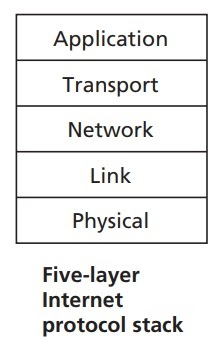
\includegraphics[width=0.25\textwidth]{images/3.jpg}
\end{center}


فرض کنید دو برنامه داریم که بر روی دو کامپیوتر جدا از طریق شبکه با هم در ارتباط هستند:

\begin{enumerate}

\item
\textbf{\lr{Application layer}}:  این لایه در واقع \lr{API} یا واسطی است که به وسیله‌ی آن این دو برنامه حرف همدیگر را می‌فهمند. مثلا برنامه نویس قرارداد (\lr{protocol}) می‌کند که برنامه اول به برنامه دوم در ابتدا یک رشته \lr{"salam"} بفرستد. سپس برنامه دوم در جواب این رشته بتواند یکی از دو رشته‌ی \lr{"Aleik"‌} و یا \lr{"Bye"} را بفرستد و اگر برنامه دوم \lr{"Aleik"} را فرستاده بود برنامه اول ...

مثلا \lr{HTTP‌} از پروتکل‌های لایه اپلیکیشن است که در وب بسیار کاربرد دارد.


\item
\textbf{\lr{Transport layer}}: این لایه پایین‌تر از لایه \lr{Application} قرار دارد (‌در واقع ارتباط بین این دو لایه از طریق سوکت (\lr{socket}) برقرار می‌شود که در مورد آن صحبت خواهد شد). همان طور که می‌دانیم، در کامپیوتر ما چندین برنامه در حال ارتباط با شبکه هستند. پس اگر برنامه اول (از کامپیوتر اول) پیامی را به سمت کامپیوتر دوم می‌فرستد، این کامپیوتر باید به نحوی بفهمد که این پیام برای کدام برنامه است. این عملیات در این لایه پیاده سازی شده است. در واقع به هر برنامه (\lr{process}) که منتظر دریافت پیام از شبکه است (\lr{listening})‌، یک عدد به اسم پورت نسبت داده می‌شود که با استفاده از آن برنامه مقصد بطور یکتا در کامپیوتر مشخص می‌شود .\lr{TCP} و \lr{UDP}، دو پروتکل این لایه محسوب می‌شوند.


\item
\textbf{\lr{Network Layer}}: حال فرض کنید برنامه اول پیامش (\lr{packet}) را فرستاد. این پیام چگونه باید به کامپیوتر مقصد برسد؟ فرایند مسیریابی (\lr{routing}) در شبکه توسط این لایه پیاده سازی شده است. در واقع هر میزبان (\lr{host})‌، یک آدرس یکتایی خواهد داشت به اسم \lr{IP address}. برای فرستادن یک بسته، برروی آن \lr{IP} مقصد برچسب می‌خورد و با سرویس‌هایی که این لایه فراهم می‌کند، این بسته به مقصد می‌رسد.

\end{enumerate}

\textbf{بیشتر بدانید:) }


در حال حاضر دو نسخه از \lr{IP} پیاده شده است که به \lr{IP} های رایج که به فرمت \lr{X.X.X.X} بوده و 32 بیتی هستند \lr{IPv4} گفته شده و به \lr{IP} هایی که به فرمت \lr{X:X:X:X:X:X:X:X} و 128 بیتی هستند \lr{IPv6} می‌گویند.

\begin{itemize}

\newpage
\item
رنج‌های \lr{IP}:

\begin{itemize}
\item
\lr{IP} های محلی: این بازه از \lr{IP} ها فقط درون همان شبکه معتبر و یکتا است و عملا خارج از اسکوپ(\lr{scope}) آن شبکه اعتبار ندارد و دیگر یکتا نیست.

\begin{enumerate}

\item
\lr{10.0.0.0} تا \lr{10.255.255.255}

\item
\lr{172.16.0.0} تا \lr{172.31.255.255}

\item
\lr{192.168.0.0} تا \lr{192.168.255.255}

\end{enumerate}

\item

\lr{IP} های عمومی: تمامی \lr{IP} ها به جز \lr{IP} محلی از این نوع هستند.

\end{itemize}

\item
 این لایه و لایه‌های بعدی بطور کلی مسئولیت مسیریابی و یافتن مسیر بهینه (با توجه به سیاست‌های شبکه) برای رسیدن هر بسته به مقصد مورد نظر با استفاده از تجهیزات (مثل سوییچ ، روتر و ...‌)‌ و پروتکل‌هایی که در این لایه و دو لایه بعد وجود دارد (\lr{IP} در این لایه و به طور مثال \lr{Ethernet} در لایه بعدی و …) را بر عهده دارند که با توجه عدم نیاز به آشنایی با لایه‌های بعدی و پروتکل‌های آن در این پروژه، در مورد لایه‌های بعد صحبتی نمی‌کنیم.
\end{itemize}

\newpage
\section*{{\titr معماری شبکه}}
\addcontentsline{toc}{section}{{\fehrestContent معماری شبکه}}

معماری شبکه به طراحی فیزیکی و منطقی نرم افزار ، سخت افزار، پروتکل‌ها و رسانه انتقال داده‌ها می‌پردازد. به زبان ساده‌تر می‌توان گفت که چگونه کامپیوترها ساماندهی شده و با هم ارتباط گرفته و چگونه وظایف به رایانه اختصاص می‌یابد.

معماری شبکه به دو نوع عمده
 \href{https://en.wikipedia.org/wiki/Peer-to-peer}{\textcolor{blue}{\underline{\lr{Peer-To-Peer}}}}
 و
  \href{https://en.wikipedia.org/wiki/Client%E2%80%93server_model}{\textcolor{blue}{\underline{\lr{Client-Server}}}}
   تقسیم می‌شود.

شبکه Peer-To-Peer شبکه‌ای است که در آن کلیه رایانه‌ها با امتیاز و مسئولیت برابر برای پردازش داده‌ها بهم متصل می‌شوند.

\begin{center}
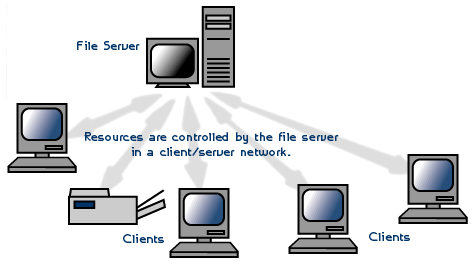
\includegraphics[width=0.5\textwidth]{images/4.png}
\end{center}


\begin{center}
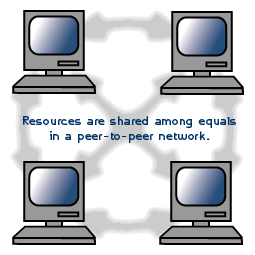
\includegraphics[width=0.5\textwidth]{images/5.png}
\end{center}

\newpage
\section*{{\titr معماری Client-Server}}
\addcontentsline{toc}{section}{{\fehrestContent معماری Client-Server}}

مدل \lr{Client-Server} که بسیاری از شبکه‌ها بر مبنای این مدل کار می‌کنند شامل یک برنامه در نقش سرور و چندین برنامه در نقش کلاینت است. منابع و اطلاعات همگی در سمت سرور نگه داشته می‌شوند و کلاینت‌ها بعد از اتصال به سرور با ارسال درخواست اطلاعات را از سرور می‌گیرند و یا اطلاعات جدید را به سرور می‌دهند.

 ارتباط کلاینت‌ها و سرور از طریق سوکت برقرار خواهد شد. سوکت بیانگر یک سر از یک ارتباط دوطرفه بین دو برنامه است. هر سوکت اطلاعات مربوط به آی پی و پورت ارتباط را نگه میدارد و دریچه ارسال و دریافت اطلاعات به آن سوی ارتباط نیز هست.
 
 اگر آدرس‌دهی یک شبکه را با فرایند آدرس‌دهی یک سیستم که بر پایه اداره پست کار می‌کند، مقایسه کنید، آن‌گاه متوجه خواهید شد که آدرس آی‌پی میزبان نقش آدرس یک ساختمان را داشته و درگاه (پورت) شبیه به شماره واحدی است که درون یک ساختمان قرار دارد و سوکت نیز مانند صندوق پست آن واحد است . یک سوکت شامل هر دو گروه آدرس آی‌پی میزبان و پورت \lr{TCP} یا \lr{UDP} مربوط به یک برنامه است که با یک علامت جداکننده این دو مقدار از یکدیگر جدا شده‌اند. (مثلا \lr{172.0.0.1:8000})

سوکت‌ها دو نوع مهم دارند:

\begin{enumerate}

\item
سوکت‌های استریم که از پروتکل \href{TCP}{\textcolor{blue}{\underline{\lr{TCP}}}} برای انتقال داده استفاده می‌کنند.

\item
سوکت‌های دیتاگرام که از پروتکل \href{https://en.wikipedia.org/wiki/User_Datagram_Protocol}{\textcolor{blue}{\underline{\lr{UDP}}}} برای انتقال داده استفاده می‌کنند.

\end{enumerate}

پروتکل \lr{TCP (transmission control protocol)} يک پروتکل ارتباط محور (\lr{connection oriented}) است و عملکرد آن بدين صورت است که براي هر پکت ارسالي توسط کامپيوتر مبدا، بايد يک پکت از سرور مقصد، مبنی بر دريافت صحيح و بدون نقص پکت دريافت کند. اگر طی زمان مشخصی اين پيام توسط مبدا دريافت نگردد، فرايند ارسال پکت مجددا تکرار خواهد شد و کاربرد آن بيشتر در مواردي است که نياز به اطمينان از صحت انتقال اطلاعات داريم. (مثل ارتباط اپلیکیشن بانکی با سرور بانک)


پروتکل \lr{UDP (User Datagram Protocol)} يک پروتکل غیر ارتباط محور (\lr{connectionless}) است. بر خلاف \lr{TCP} در اين پروتکل هيچ گونه پيامي مبني بر دريافت پکت از سوي سرور ارسال نشده و بيشتر در مواردی مانند انتقال صوت يا ويدئو که پهناي باند در اين موارد از اهمیت بالایی برخوردار است بكار می‌رود زيرا در صورت استفاده از پروتکل \lr{TCP}، ترافيک هر پيام تایید به ازای دریافت پکت، خود باعث اشغال پهناي باند خواهد شد.

\section*{{\titr شبکه در جاوا}}
\addcontentsline{toc}{section}{{\fehrestContent شبکه در جاوا}}

کلاس \lr{Socket} و \lr{ServerSocket} که در کلاس و حل تمرین نحوه استفاده و پیاده‌سازی آن تدریس شده، از نوع \lr{TCP} هستند. برای آشنایی بیش‌تر می‌توانید به
 \href{اینجا}{\textcolor{blue}{\underline{{اینجا}}}} و
  برای هندل کردن همزمان چند کلاینت به
   \href{https://medium.com/martinomburajr/java-create-your-own-hello-world-server-2ca33b6957e}{\textcolor{blue}{\underline{{اینجا}}}}
    مراجعه کنید.
    
همچنین برای آشنایی با پیاده سازی پروتکل \lr{HTTP} در جاوا می‌توانید به
 \href{این لینک }{\textcolor{blue}{\underline{{این لینک }}}}
 مراجعه کنید.


از آنجایی که در پروژه شما سرعت و حجم انتقال داده‌ها اهمیت چندانی ندارد نیازی به استفاده از سوکت udp ندارید اما برای آشنایی بیشتر با پیاده سازی این مدل می‌توانید به لینک های زیر مراجعه کنید.

\begin{flushleft}
\href{https://www.baeldung.com/udp-in-java}{\textcolor{blue}{\underline{\lr{A Guide To UDP In Java}}}}
\end{flushleft}

\begin{flushleft}
\href{TCP vs UDP - Difference and Comparison}{\textcolor{blue}{\underline{\lr{TCP vs UDP - Difference and Comparison}}}}
\end{flushleft}


به طور خلاصه ارتباط بین سرور و کلاینت (مدل \lr{TCP}) به طریق زیر صورت می‌گیرد:

\begin{enumerate}

\item
سرور یک سوکت بر روی پورت مثلا \lr{6666} می‌سازد و به آن گوش می‌کند:

\begin{latin}

\begin{lstlisting}{java}
//Server side
ServerSocket ss=new ServerSocket(6666);  

\end{lstlisting}

\end{latin}

\item
کلاینت نیز یک سوکت می‌سازد و روی همان پورت درخواست اتصال می‌دهد:

\begin{latin}

\begin{lstlisting}{java}
//Server side
//Client side
Socket s=new Socket("localhost",6666)	;
//localhost == 127.0.0.1
 

\end{lstlisting}

\end{latin}

\item
سرور با دریافت درخواست اتصال آن‌ را تایید می‌کند و دو طرف به هم وصل می‌شوند:


\begin{latin}

\begin{lstlisting}{java}
//Server side
Socket s=ss.accept();

\end{lstlisting}

\end{latin}

\item
دو طرف از طریق سوکت سمت خودشان شروع به تبادل داده می‌کنند:


\begin{latin}

\begin{lstlisting}{java}
//Client side
DataOutputStream dout=new DataOutputStream(s.getOutputStream());  dout.writeUTF("Hello Server");  			
\end{lstlisting}

\end{latin}

\begin{latin}

\begin{lstlisting}{java}
//Server side
DataInputStream dis=new DataInputStream(s.getInputStream());
String  str=(String)dis.readUTF();  

\end{lstlisting}

\end{latin}



\end{enumerate}

دقت کنید که پورتی که سرور می‌خواهد استفاده کند نباید در اختیار(bind) برنامه دیگری باشد، برای فهمیدن اینکه چه پورت‌هایی توسط سیستم یا برنامه های دیگر در حال استفاده هستند می‌توانید به این لینک ها مراجعه کنید:
\href{https://www.howtogeek.com/howto/28609/how-can-i-tell-what-is-listening-on-a-tcpip-port-in-windows/}{\textcolor{blue}{\underline{{ ویندوز}}}}
  ،
   \href{https://www.cyberciti.biz/faq/unix-linux-check-if-port-is-in-use-command/}{\textcolor{blue}{\underline{{لینوکس}}}}


\section*{{\titr معماری Peer-To-Peer}}
\addcontentsline{toc}{section}{{\fehrestContent معماری Peer-To-Peer}}

برای مطالعه در مورد این معماری که از موارد امتیازی این فاز است، به \textcolor{CustomColor}{داک \lr{P2P}} مراجعه کنید.


\section*{{\titr Token Authentication }}
\addcontentsline{toc}{section}{{\fehrestContent Token Authentication }}

\lr{Token} یک کلید برای ارتباط بین کلاینت و سرور است. برای هر کاربر پس از احراز هویت توسط نام کاربری و رمز عبور یا هر روش دیگر، یک \lr{Token}  از سمت سرور مشخص می‌شود که از آن به بعد، پیام‌های ارسالی توسط کاربر به وسیله ی آن \lr{Token} در سرور شناسایی می‌شوند. این \lr{Token} ها می‌توانند محدودیت زمانی استفاده داشته باشند و برای رعایت امنیت باید پس از هر بار ورود دوباره‌ی کاربر \lr{Token} جدیدی به او اختصاص داده شود.

پیاده سازی توکن در ارتباط بین کلاینت و سرور فروشگاه از موارد امتیازی این فاز است.

برای مطالعه بیشتر در مورد توکن به این لینک مراجعه کنید:


\begin{center}
\href{https://scotch.io/tutorials/the-ins-and-outs-of-token-based-authentication}{\textcolor{blue}{\underline{\lr{The Ins and Outs of Token Based Authentication}}}}

\end{center}

\end{document}







